Generally speaking, in a competitive environment, agents pursuit 2 objectives: trying to weaken an adversary, and gain
as much profit as possible whatever the form that profit may take. To create a meaningful illustration of the approach,
it is proposed to consider the following multi agent environment model. There are 2 adversarial teams (swarms), plus a
special type of agents called "resource". The environment has spatial qualities, which enables distance-driven
reasoning. Agents move in the environment, attack each other, and gather resources spawning occasionally in a manner
unpredictable for individual agents.

Every team has a resource value associated with it, whilst every agent has that of energy. Every action or interaction
between agents can be expressed in terms of gain or loss of energy, resource, or both. In a span of one iteration, every
agent may be idle while restoring energy, or either run avoiding troubles, gather resource, or try to attack enemies.

Among the plethora of possible AHP-based interpretations of this environment in terms of strategic / tactic reasoning,
we propose the one that defines it in terms of "invasive" versus "secure" (or "safe") strategies (Figure
\ref{fig:prefgraph-simulation}).

\begin{figure}[hbt!]
    \centering
    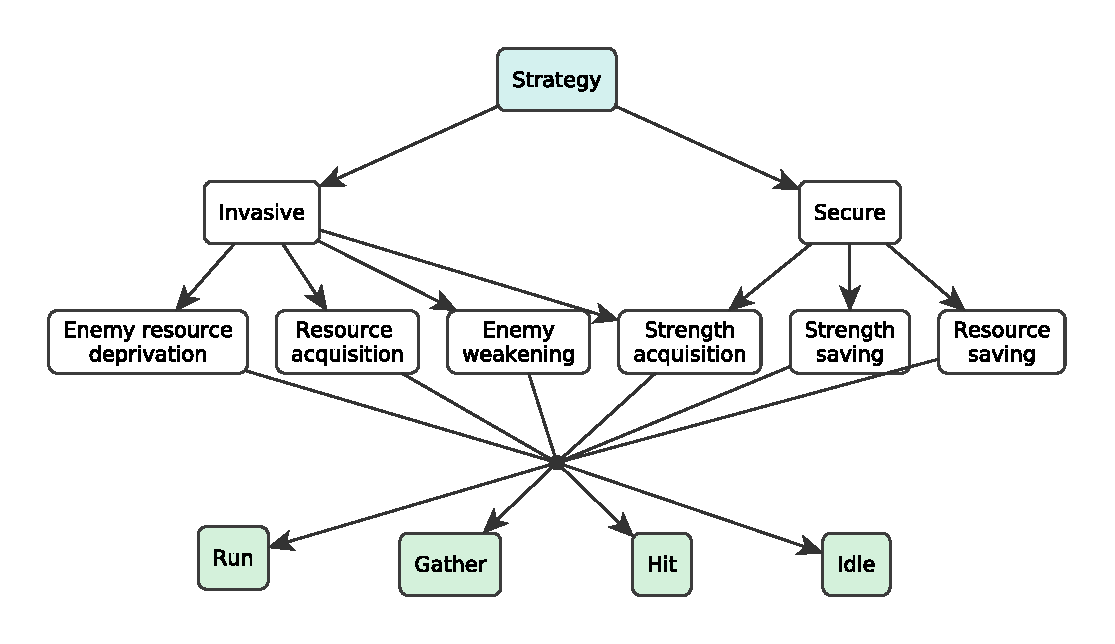
\includegraphics[width=0.8\textwidth]{prefgraph.eps}

    \caption{\small Preference graph}
    \label{fig:prefgraph-simulation}
\end{figure}

The "invasive" one is more external-oriented, as it comprises "sub-aspects" as "enemy weakening" and "enemy resource
deprivation". "Secure" strategy expresses goals oriented towards saving a domestic swarm. They both share the common
sub-aspect called "strength acquisition", because arguably it impacts both expansionistic and defensive approaches. But
of course this depends on a particular implementation's details.

Possible agents' actions then get assessed in terms of these lower-level strategies (drawn in green) every time before
an agent makes a decision.